\documentclass[a4paper]{article}

\usepackage{geometry}
 \geometry{
 a4paper,
 total={170mm,257mm},
 left=20mm,
 top=20mm,
 }
 
\usepackage[english]{babel}
\usepackage[utf8]{inputenc}
\usepackage{amsmath}
\usepackage{graphicx,caption,subcaption,float}
\usepackage[colorinlistoftodos]{todonotes}

\title{APC 524 / AST 506 / MAE 506 Software engineering for scientific computing
\\Assignment 4: Parallel programming with OpenMP and MPI}

\author{Hao Zhang, MAE, haozhang@princeton.edu}

\date{\today}

\begin{document}
\maketitle

    \section{Computation time}
<<<<<<< HEAD
   For the sake of time, we only consider grid size $nx=64,128,256$. It's found that OpenMP and MPI produce nearly-linear speed-up. With the increase of threads, the perfect linear speed-up is actually limited by process that can not be (easily) parallelized(i.e., I/O process).
=======
    It's found that OpenMP and MPI produces nearly-linear speed-up. With the increase of threads, the perfect linear speed-up is actually limited by process that can not be (easily) parallelized(i.e., I/O process).
>>>>>>> e42861b141236da8b88833f527a2ee1c0c5a4535
      \begin{figure}[H]
            \centering 
            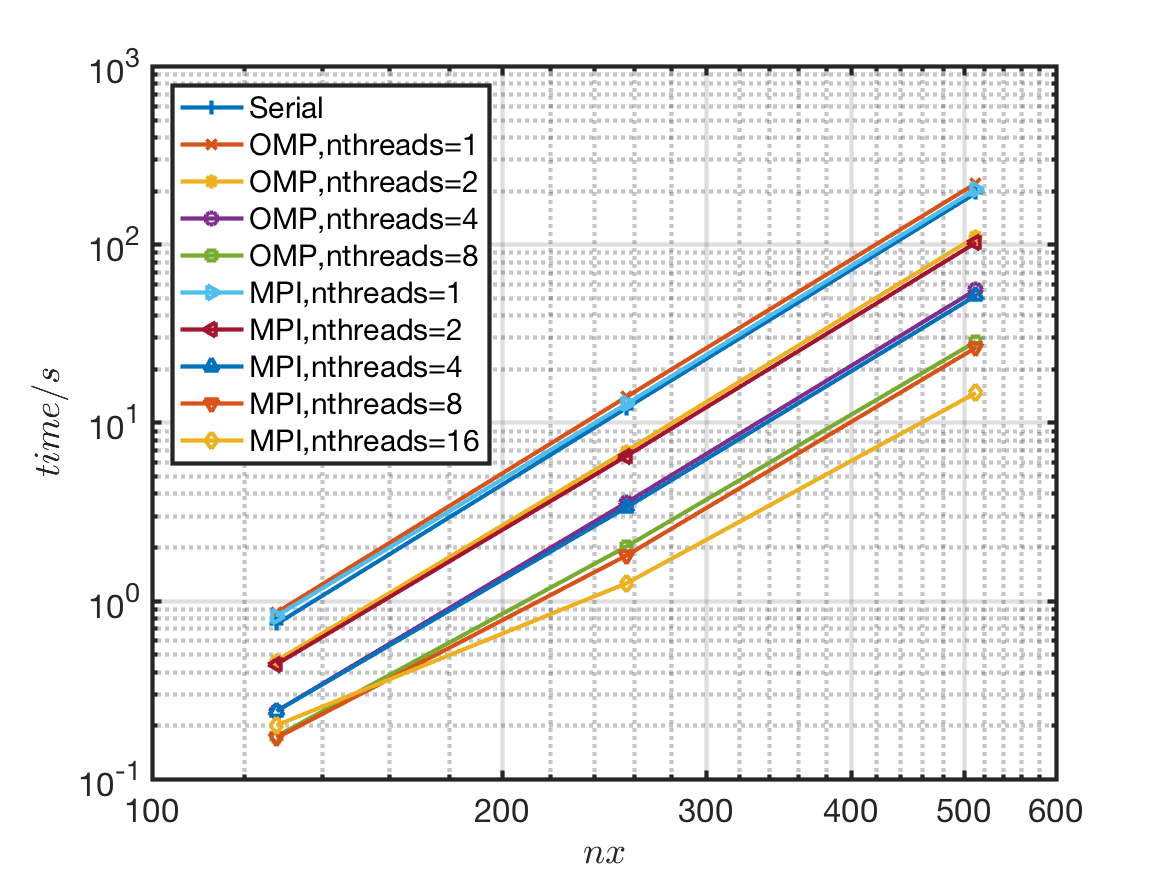
\includegraphics[width=0.8\textwidth]{./Figure/computation_time.png} 
        \caption{Computation time of serial, OpenMP, MPI (with various threads) with respect to grid size $nx=64,128,256$. All simulation is run on Adroit cluster.}
    \end{figure}
    
    Average temperature is not reported here, but they are almost the same ($T_{mean} \approx 0.4930$) for all runs.
    
\section{Single thread, Serial vs OpenMP vs MPI}
With a single thread, serial, OpenMP, and MPI takes almot the same computation time. The temperature field are visually identical.
      \begin{figure}[H]
        \centering
        \begin{subfigure}[b]{0.32\textwidth}   
            \centering 
            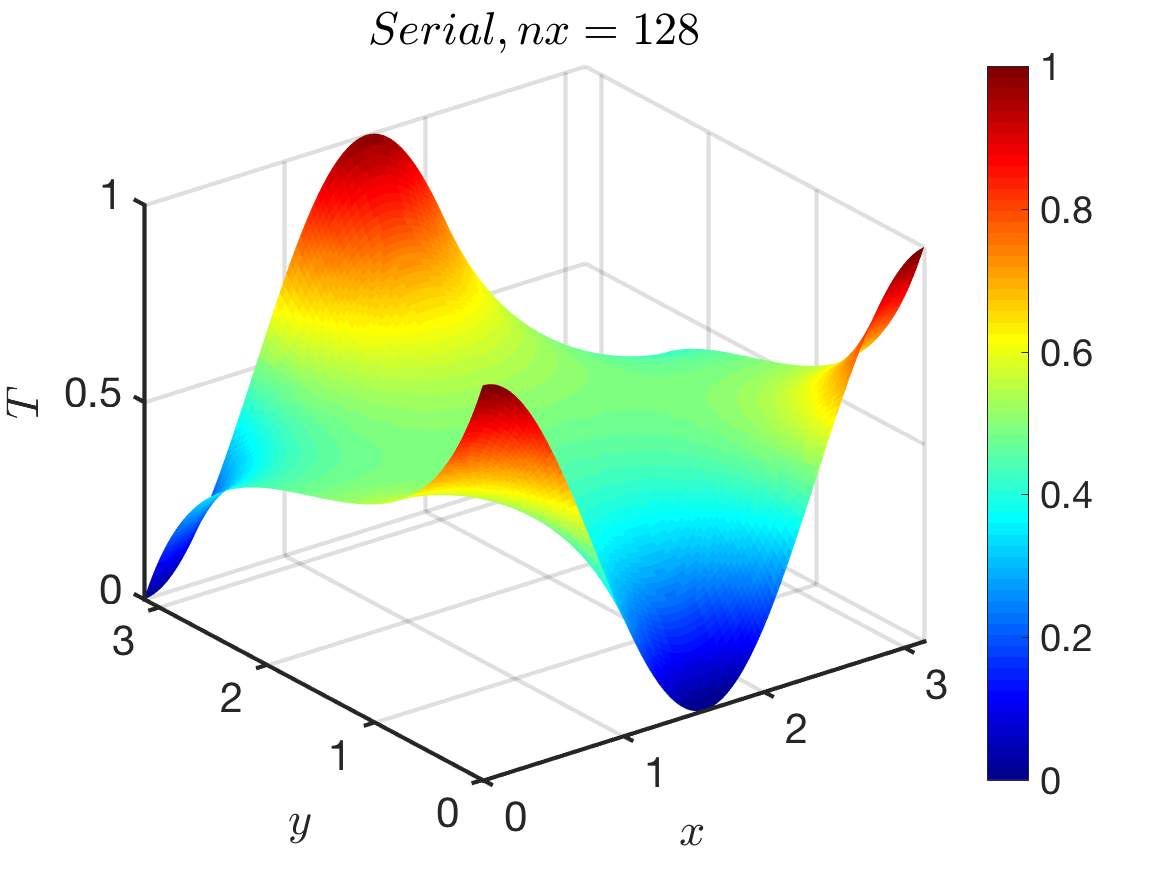
\includegraphics[width=\textwidth]{./Figure/heat_serial_nx128.png} 
        \end{subfigure}
        \
        \begin{subfigure}[b]{0.32\textwidth}   
            \centering 
            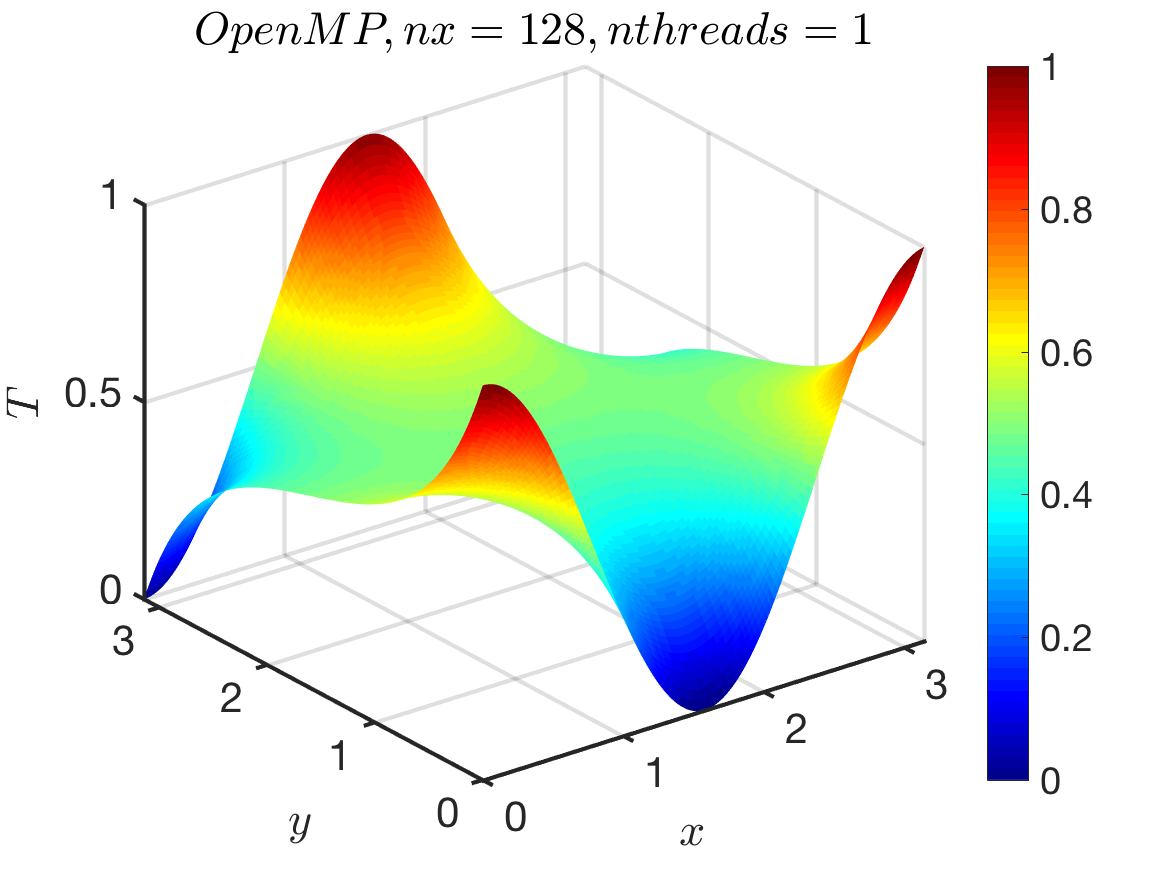
\includegraphics[width=\textwidth]{./Figure/heat_omp_nx128_nth1.png}  
        \end{subfigure}
        \
                \begin{subfigure}[b]{0.32\textwidth}   
            \centering 
            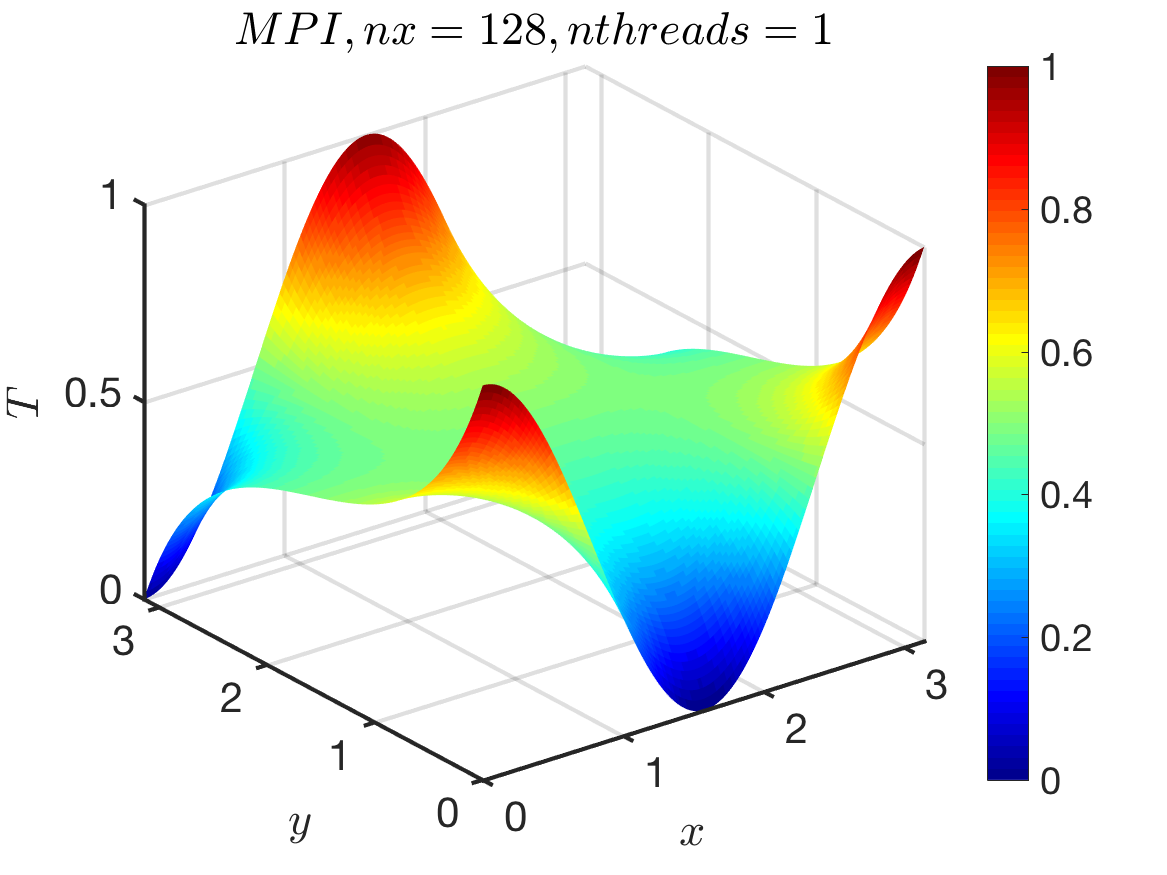
\includegraphics[width=\textwidth]{./Figure/heat_mpi_nx128_nth1.png} 
        \end{subfigure}
        \caption{Temperature field computed by serial, OpenMP, and MPI with a single thread, grid size $128\times128$}
    \end{figure}
    
    \section{OpenMP, multiple threads}
    To parallel serial code with OpenMP, we only need to add a few new lines before the for loop. A header file "omp.h" also needs to be included. It's extremely easy to implement, and the gain is large(depending on the number of threads in the processor).
    
          \begin{figure}[H]
        \centering
        \begin{subfigure}[b]{0.32\textwidth}   
            \centering 
            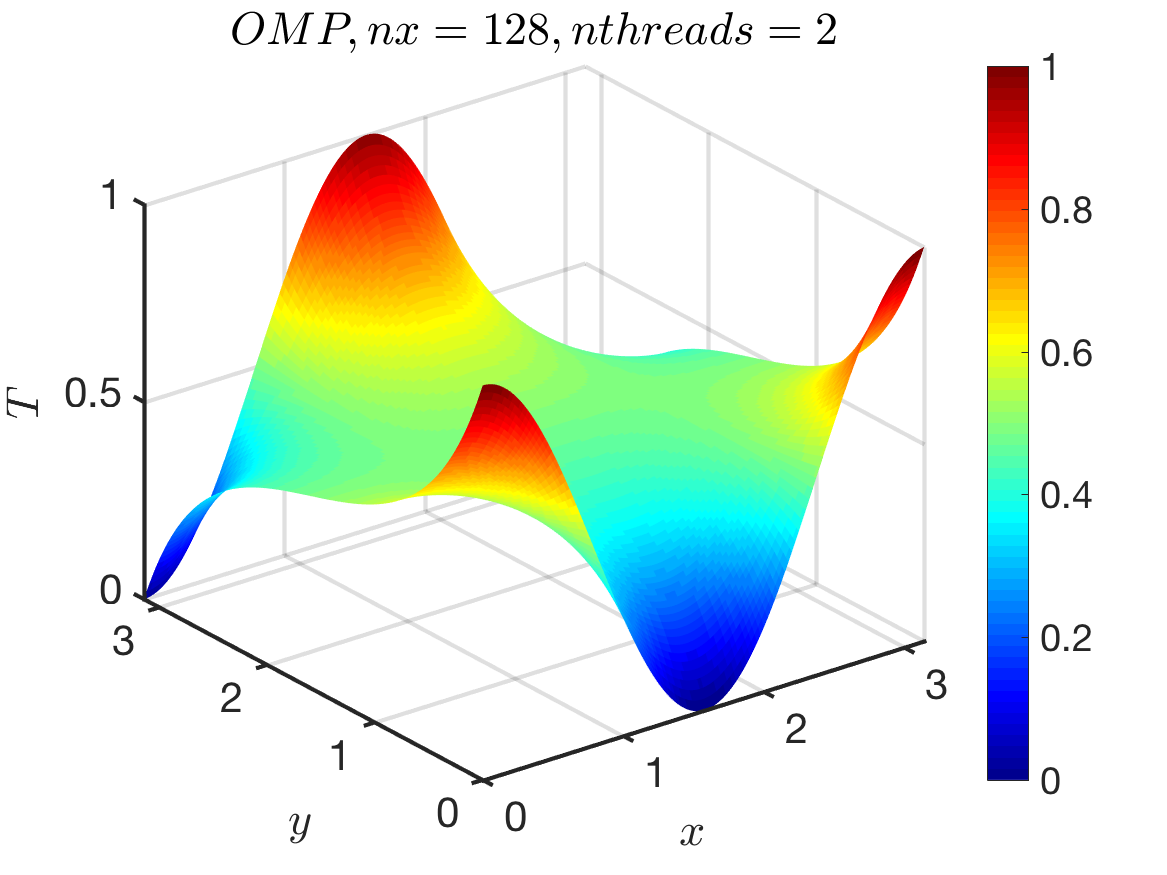
\includegraphics[width=\textwidth]{./Figure/heat_omp_nx128_nth2.png} 
        \end{subfigure}
        \
        \begin{subfigure}[b]{0.32\textwidth}   
            \centering 
            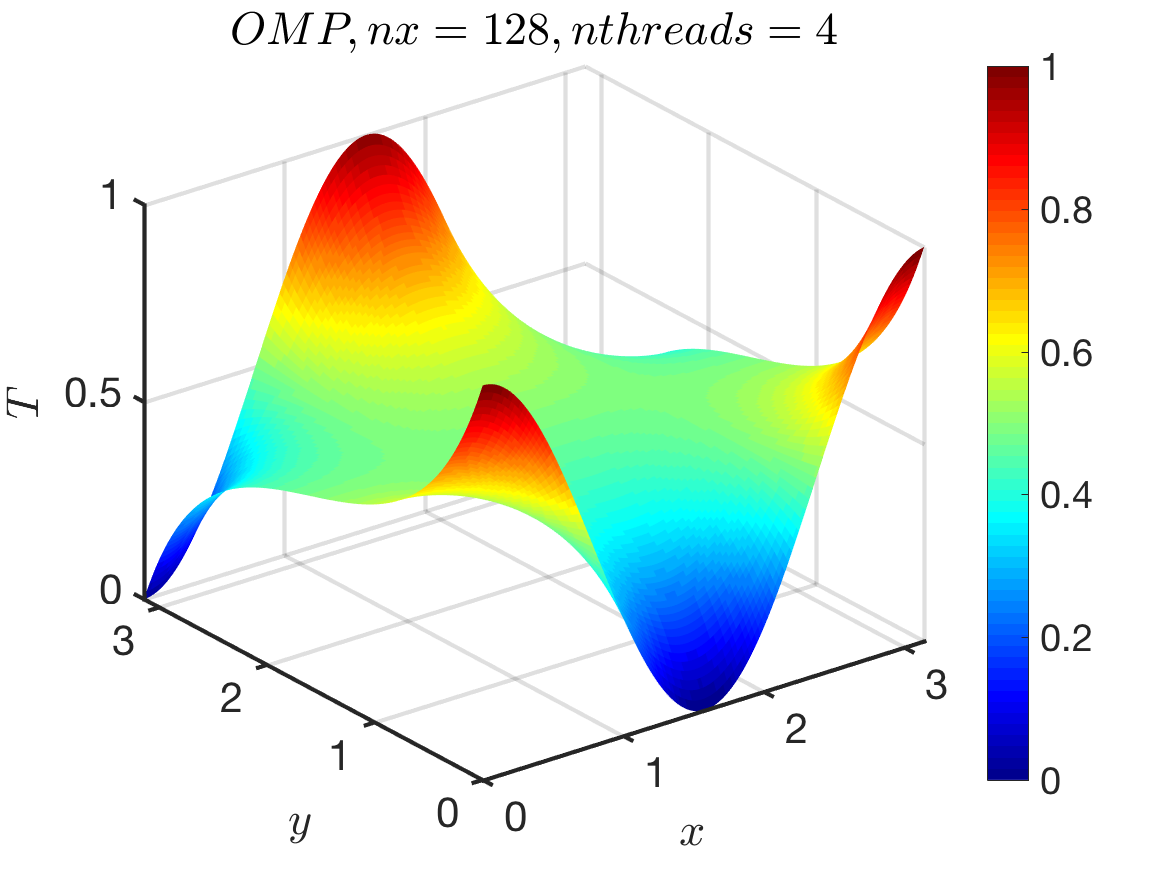
\includegraphics[width=\textwidth]{./Figure/heat_omp_nx128_nth4.png}  
        \end{subfigure}
        \
                \begin{subfigure}[b]{0.32\textwidth}   
            \centering 
            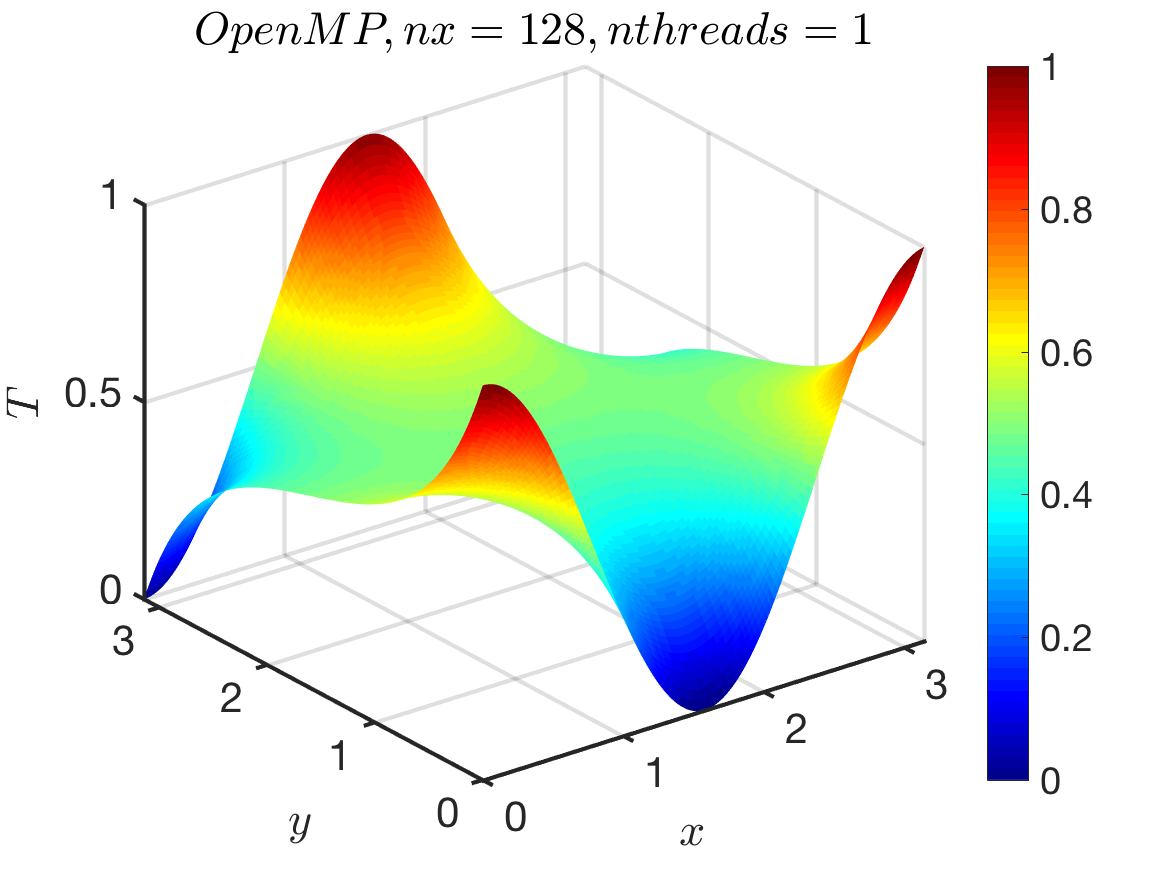
\includegraphics[width=\textwidth]{./Figure/heat_omp_nx128_nth8.png} 
        \end{subfigure}
        \caption{Temperature field computed by OpenMP with nthreads = 2,4,8, grid size $128\times128$}
    \end{figure}
    
    \section{MPI, multiple threads}
    When MPI is used to parallelize the updating step, domain decomposition is ultilized to divide tasks into small chunks. The boundary points are passed between various threads, by calling function MPI-Send() and MPI-Recv().
              \begin{figure}[H]
        \centering
        \begin{subfigure}[b]{0.32\textwidth}   
            \centering 
            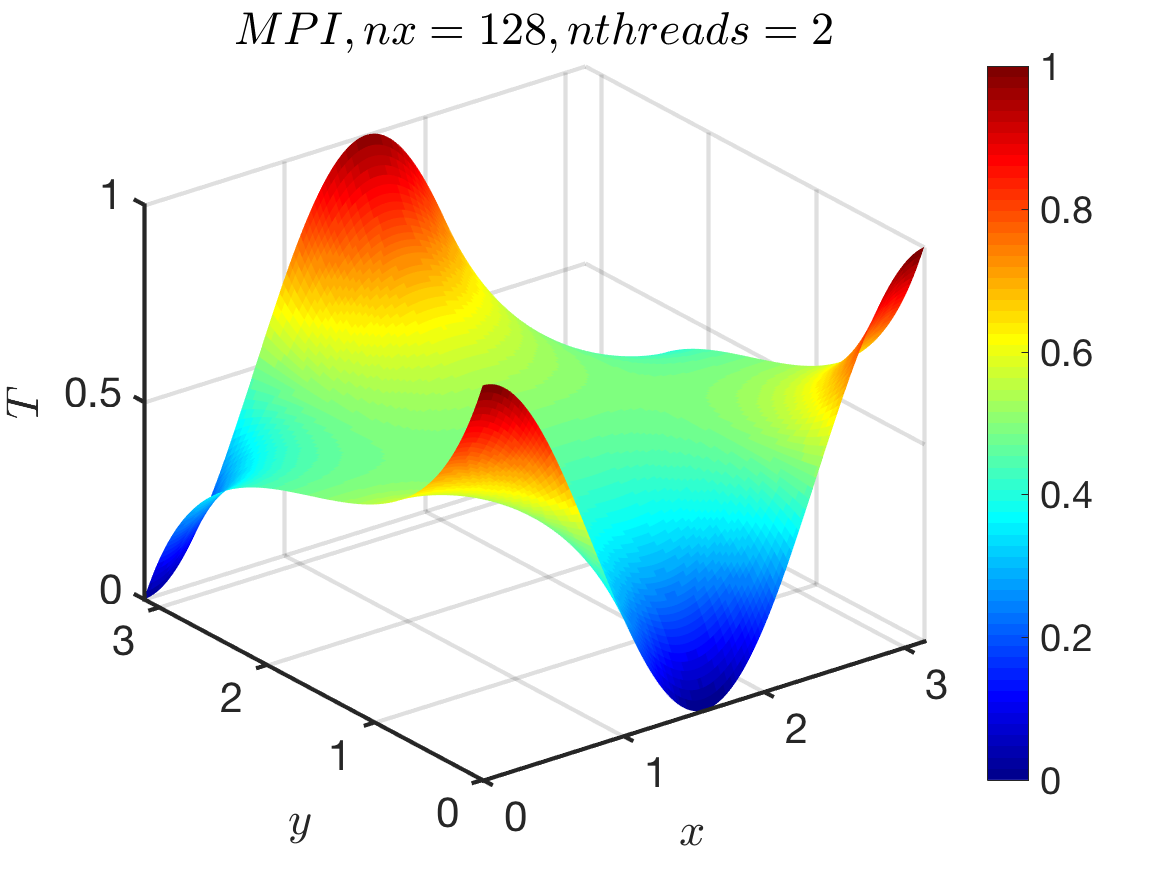
\includegraphics[width=\textwidth]{./Figure/heat_mpi_nx128_nth2.png} 
        \end{subfigure}
        \
        \begin{subfigure}[b]{0.32\textwidth}   
            \centering 
            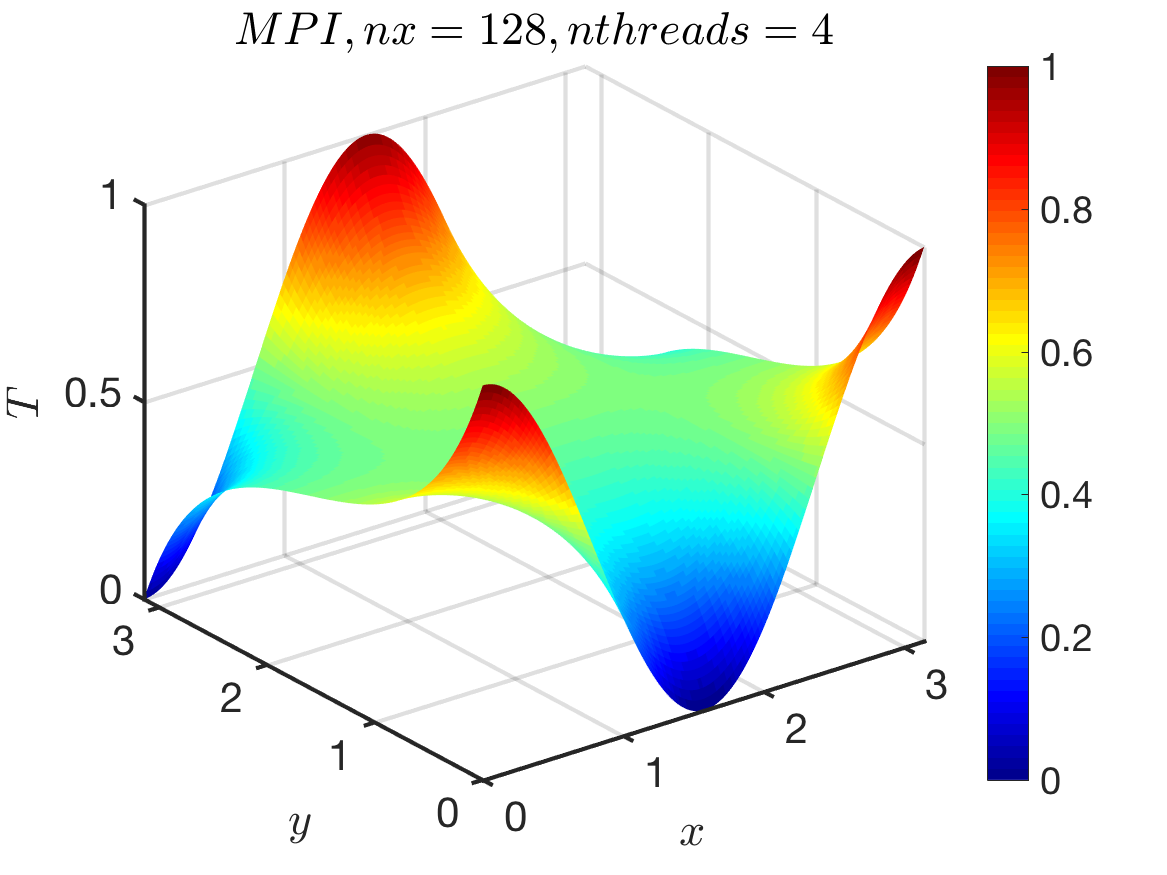
\includegraphics[width=\textwidth]{./Figure/heat_mpi_nx128_nth4.png}  
        \end{subfigure}
        \
                \begin{subfigure}[b]{0.32\textwidth}   
            \centering 
            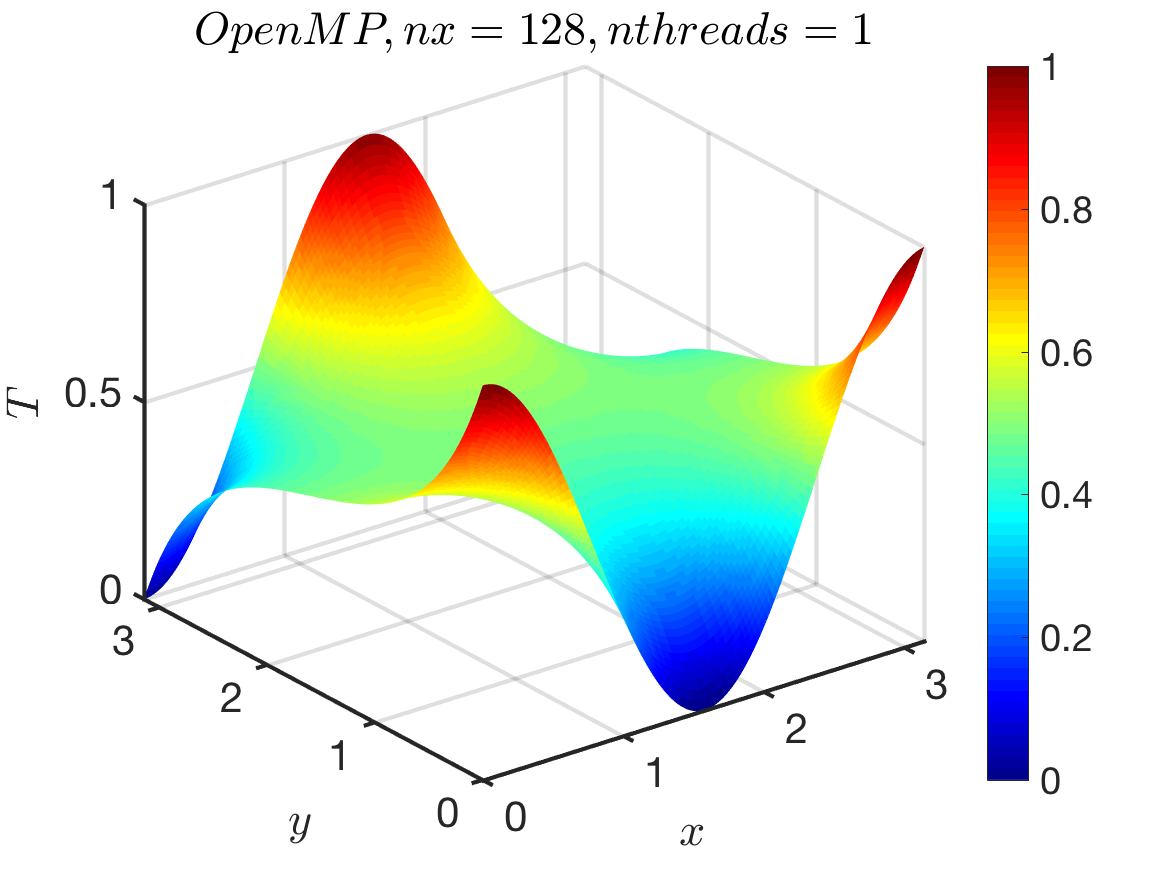
\includegraphics[width=\textwidth]{./Figure/heat_mpi_nx128_nth8.png} 
        \end{subfigure}
        \caption{Temperature field computed by MPI with nthreads = 2,4,8, grid size $128\times128$}
    \end{figure}
    
    \section{OpenMP vs MPI}
OpenMP is very easy to use, we only need to add a few lines to the serial code and include "omp.h" header file. However, OpenMP only works on a single processor, so speed-up is limited by the number of threads available.\\

MPI takes more effort to implement, and it's more error-prone. However, MPI in principle works for much more systems/hardwares architecture. For example, it can make full use all the processors on one machine, and even combine the computation power of multiple machines.
    
\end{document}